\chapter{Analysis and specification of needs }

\section{Introduction}

The success of any project depends on the quality of its outset. Therefore, the step of specifying the needs constitutes the starting base of our work; it must unequivocally describe the application to be developed. To ensure the expected objectives, it is essential that we achieve a clear view of the various anticipated needs of our project. In this chapter, we will identify the expected functionalities of the module by defining the various use cases. 

\section{Identification of stakeholders}

We start by identifying the actors involved in our solution. An actor is a person or component that interacts with the system. In our case, we have two actors:

\begin{itemize}
    \item The client: any individual
    \item The administrator: person responsible for the maintenance and 
        monitoring of a website or server on the Internet."
\end{itemize}
 \\
 
\section{Needs analysis }

\subsection{Functional needs analysis }

The analysis of functional needs translates the desired requirement by the client into functionalities achievable by our application.

The client can:

\begin{itemize}
    \item Register in the application
    \item Log into the application
    \item View reservation history
    \item Add a reservation
    \item Track the progress of reservation statuses
\end{itemize}
        The administrator can:

\begin{itemize}
    \item Log into the application
    \item Process reservations
    \item View reservations.

\end{itemize}

\subsection{The non-functional requirements }

Non-functional requirements represent the implicit requirements that the system must meet. For the proper functioning of our project, we have identified the following non-functional requirements:

\begin{itemize}
    \item \textbf{Usability:} ease of learning and use.
    \item \textbf{Efficiency:} it is imperative to minimize the processing time.
    \item \textbf{Utility:} the site must be efficient through its functionalities, and it 
        must meet all user requirements optimally. 
        \item \textbf{Extensibility:} the ease with which new functionalities can be added. 
\end{itemize}
 
\section{Modeling of requirements }

We have opted for the object-oriented method to specify our client's requirements. In this section, we present the use case diagrams.

\subsection{General use case diagram }

 The use case diagram highlights the interaction between the system and the various actors. Each use case designates a functionality of the system. 
\begin{figure}[H]
   \centering
    %\includegraphics[scale=0.5]{images/trasfvs.jpg}
    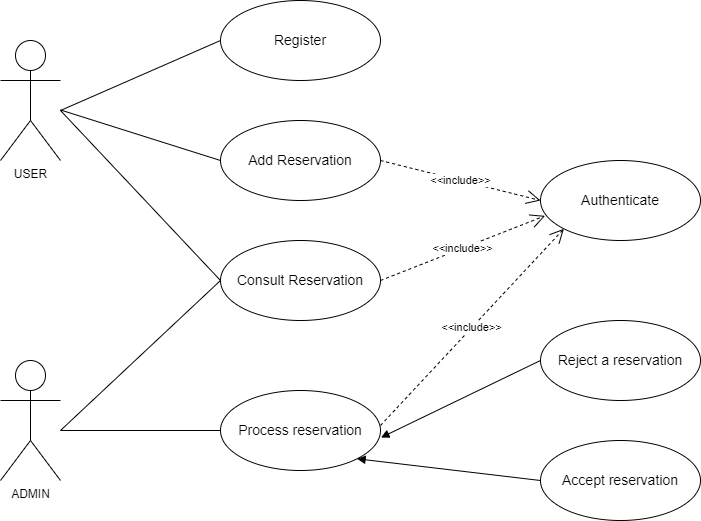
\includegraphics[width=6cm,height=6cm]{images/usecase.drawio.png}
    \caption{General use case diagram}
    \label{General use case diagram}
\end{figure}

In order to clarify the cases represented in the previous diagram, we create the following tables that contain a brief description of each use case. 
    
\textbf{• \textbf{Textual description for the use case "authenticate" }}

\begin{table}
    \centering
    \begin{tabular}{|c|l|} \hline 
         Title& Authenticate\\ \hline 
         Resume& Allow platform users to authenticate to access it.\\ \hline 
         Actors& User and Admin\\ \hline 
         Precondition&The user already has an account.\\\hline \hline 
         Nominal scenario& 1- The user enters their email address and password.\\ \hline 
 &2- The system checks the existence of the account in the DB by email.\\ \hline 
 &3- The system verifies the correspondence of the email with the pwd.\\ \hline 
 &4- Upon success, the user is authenticated.\\\hline \hline 
         Alternate scenario& E1: Account not found\\ \hline 
 &1- The system displays an error message.\\
 &2- The scenario continues from 1-\\\hline \hline 
 &E2: Incorrect password\\ \hline 
 &1- The system displays an error message'incorrect pwd or email adr'.\\ \hline
    \end{tabular}
    \caption{Textual description for the use case "authenticate"}
    \label{Textual description for the use case "authenticate"}
\end{table}

\textbf{• \textbf{Textual description for the use case "Process reservation" }}

\begin{table}
    \centering
    \begin{tabular}{|c|l|} \hline 
         Title& Process reservation\\ \hline 
         Resume& Allow the application administrator to manage complaints.\\ \hline 
         Actors& Admin\\ \hline 
         Precondition&The user is authenticated as an administrator.\\\hline \hline 
         Nominal scenario& 1- Consult reservation list.\\ \hline 
 &2- Choose a reservation to edit.\\ \hline 
 &3- Change reservation status"In progress/closed/rejected".\\\hline
    \end{tabular}
    \caption{Textual description for the use case "Process reservation" }
    \label{Textual description for the use case "Process reservation" }
\end{table}

\textbf{• \textbf{Textual description for the use case "Add reservation" }}

\begin{table}
    \centering
    \begin{tabular}{|c|l|} \hline 
         Title& Add reservation\\ \hline 
         Resume& Allow platform users to add reservation.\\ \hline 
         Actors& User \\ \hline 
         Precondition&The user is authenticated as a client\\\hline \hline 
         Nominal scenario& 1- The user clicks on "add resrvation"\\ \hline 
 &2- The system displays the reservation form\\ \hline 
 &3- The user fills out the form\\ \hline 
 &4- The user clicks on submit\\ \hline 
 &5- If successful, the reservation is successfully added.\\\hline \hline 
         Alternate scenario& E1: A field in the form is missing\\ \hline 
 &1- The system displays an error message indicating the problem.\\ \hline 
 &2- The user rectifies the error, and the scenario continues from 3.\\ \hline
    \end{tabular}
    \caption{Textual description for the use case "Add reservation"}
    \label{Textual description for the use case "Add reservation"}
\end{table}

\textbf{• \textbf{Textual description for the use case "Register " }}

\begin{table}
    \centering
    \begin{tabular}{|c|l|} \hline 
         Title& Register\\ \hline 
         Resume& Allow platform users to create an account.\\ \hline 
         Actors& User \\ \hline 
         Precondition&User have no account\\\hline \hline 
         Nominal scenario& 1- The user clicks on "Create account"\\ \hline 
 &2- The system displays the account creation form\\ \hline 
 &3- The user fills out the form and clicks on submit\\ \hline 
 &4- The system validate informations and inputs \\ \hline 
 &5- If successful, the account is successfully created.\\\hline \hline 
         Alternate scenario& E1: A field in the form is missing\\ \hline 
 &1- The system displays an error message indicating the problem.\\ \hline 
 &2- The user rectifies the error, and the scenario continues from 3.\\ \hline
 &E2: The client cancels\\\hline
    \end{tabular}
    \caption{Textual description for the use case "Register "}
    \label{Textual description for the use case "Register"}
\end{table}

\textbf{• \textbf{Textual description for the use case "Consult reservation " }}

\begin{table}
    \centering
    \begin{tabular}{|c|l|} \hline 
         Title& Consult reservation\\ \hline 
         Resume& Allow application users to view reservations.\\ \hline 
         Actors& User and Admin\\ \hline 
         Precondition&The user is authenticated\\\hline \hline 
         Nominal scenario& 1- if User : consult his own reservations\\ \hline 
 &2- if Admin : consult all reservations\\\hline
    \end{tabular}
    \caption{Textual description for the use case "Consult reservation "}
    \label{Textual description for the use case "Consult reservation"}
\end{table}


\section{Conclusion}
This chapter allowed us to cover the various functional and non-functional requirements that our solution must meet. We have also detailed these requirements through the use case diagram, in order to proceed to the design of our application, which will be presented in the next chapter. 